\section{Wire Antennas}
\subsection{Field Calculation}
\begin{itemize}
    \itemsep0pt
    \item \textbf{Strategy:} Enclose the whole wire by a closed Huygens surface and introduce equivalent electric and magnetic Huygens currents according to the tangential fields on the Huygens surface.
\end{itemize}

\subsection{Straight-Lined Dipoles and Monopoles}
\begin{tabular}{cc}
    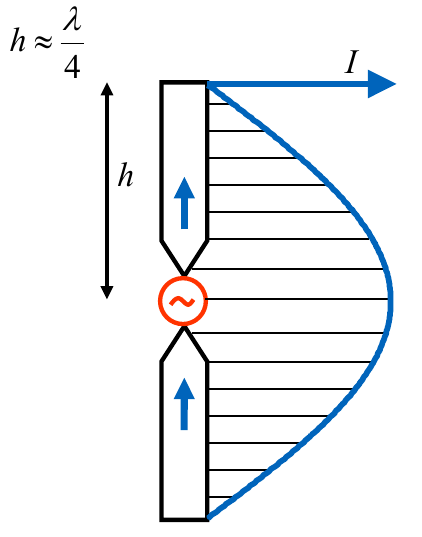
\includegraphics[width=3cm]{content/aawp/pictures/half_wave_dipole.png} &\
    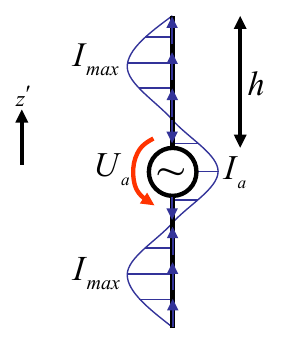
\includegraphics[width=3cm]{content/aawp/pictures/general_length_dipole.png}\\
    \textbf{Half-wave Dipole} &\
    \textbf{General-length Dipole}
\end{tabular}
\begin{center}
     \noindent\fbox{%
        \parbox{6.5cm}{%
            \hspace{1cm}\textbf{Far-field} of a \textbf{half-wave dipole:}
            \begin{align*}
                &E_\vartheta = jI_a \, \dfrac{Z_F}{2\pi} \dfrac{e^{-jkr}}{r} C(\vartheta),\\
                &C(\vartheta) = \dfrac{\cos\left(\dfrac\pi2 \cos\vartheta\right)}{\sin\vartheta}
            \end{align*}
        }}
\end{center}
\begin{itemize}
    \itemsep0pt
    \item Radiation resistance $R_r$ and Directivity $D$ of a dipole antenna:
        \begin{equation*}
            R_r = \dfrac{Z_F}{\pi} 0.61 \approx \SI{73.1}{\Omega} = Z_d
        \end{equation*}
        \begin{equation*}
            D \approx \SI{2.51}{dBi}
        \end{equation*}
    \item Dipoles of general length:
        \begin{align*}
            I(z^\prime) &= I_{\mathrm{max}} \sin\left(k (h - |z^\prime|)\right)\\
            C(\vartheta) &= \dfrac{\cos(k h \cos(\vartheta)) - \cos(k h)}{\sin(\vartheta) (1 - \cos(k h))}
        \end{align*}
    \item \textit{Monopole Antenna} has $2\times$ the directivity
\end{itemize}

\subsection{Folded Dipole}
\begin{itemize}
    \itemsep0pt
    \item \(Z_{fd} = 4 Z_d\)
    \item Its radiation characteristic $C(\cdot)$ similar to $\lambda/2$-dipole
\end{itemize}

\subsection{Baluns (Balanced - Unbalaced)}
\begin{tabular}{cc}
    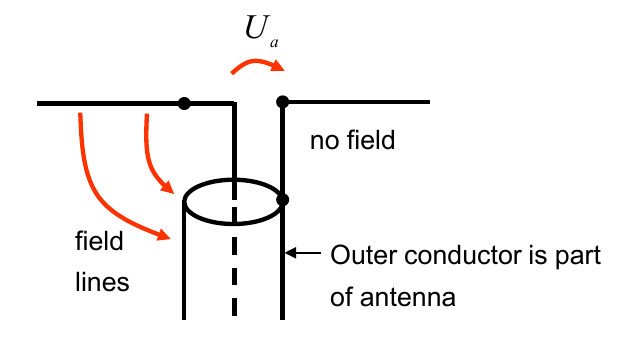
\includegraphics[width=4cm]{content/aawp/pictures/unbalanced_dipole_feed.png} &\
    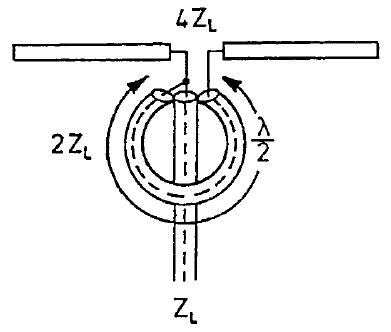
\includegraphics[width=2.7cm]{content/aawp/pictures/coaxial_half_wave_line_balun.png}\\
    \textbf{Unbalanced Dipole Feed} &\
    \parbox{3cm}{\textbf{Coaxial Half-wave Line Balun}}
\end{tabular}
\begin{itemize}
    \itemsep0pt
    \item \textbf{Purpose:} Feeding of symmetric (balanced) antenna (e.g. dipole, folded dipole) with an unbalanced transmission line (e.g. coax cable, micro strip line)
    \item Prevents the following:
        \begin{itemize}
            \item \textit{Sheath Current} (Mantelströme)
            \item Distortion of radiation pattern and input impedance
        \end{itemize}
\end{itemize}

\subsection{Helical Antennas}
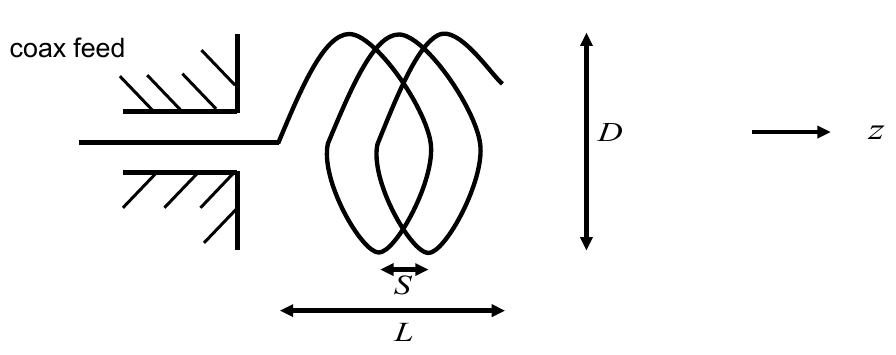
\includegraphics[width=7cm]{content/aawp/pictures/helical_antenna.png}\\
\begin{enumerate}
    \item \textbf{Normal mode} (\(D, L \ll \lambda \implies\) constant current on helix, \textit{broadside radiation})
    \item \textbf{Axial Helix mode} (\(\frac{3}{4}\lambda \leq \pi D \leq \frac{4}{3}\lambda \implies\) approx. one wavelength on the circumference of each loop, \textit{axial radiation}):
        \begin{itemize}
            \itemsep0pt
            \item Pitch angle \(\alpha = \ang{12}..\ang{15} \implies S \approx \frac{\lambda}{4}\)
            \item Circular (elliptical) polarization
            \item Good bandwidth, efficiency, gain up to \SI{15}{dBi}
        \end{itemize}
\end{enumerate}
